\documentclass[12pt,a4paper]{article}
\usepackage[utf8]{inputenc}
\usepackage[spanish]{babel}
\usepackage[left=2.5cm,right=2.5cm,top=2cm,bottom=3.5cm]{geometry}
\usepackage{float}
\usepackage{graphicx} 
\usepackage{enumitem}
\usepackage{booktabs}
\usepackage{amsmath}
\usepackage[hidelinks]{hyperref}
\usepackage{parskip}
\setlength{\parindent}{1.27cm} 

\begin{document}

\begin{titlepage}
	\centering
	
\includegraphics[width=0.4\textwidth]{../../resources/logos/Nuevo-logo-UTB-1.png}\par\vspace{1.5cm} 
	{\scshape\LARGE\textbf{Universidad Tecnológica de Bolívar} \par}
	\vspace{1.5cm}
    \rule{\linewidth}{0.2 mm} \\[0.4 cm]
	{\huge\bfseries Análisis experimental y numérico de una caída libre por ajuste de datos \par} 
    \rule{\linewidth}{0.2 mm} \\[1.0 cm]
	\vspace{0.5cm}
	
	{\large\textbf{Actividad 1 - Primer corte} \par}
	\vspace{1.5cm}

    \centering{\emph{\textbf{Estudiantes:}}\\
        German De Armas Castaño \\ 
        Angel Vega Rodriguez \\
        Michael Taboada Naranjo\\}
        
    \vspace{1 cm}
    \centering{\emph{\textbf{Profesor:}}\\
        David Sierra Porta\\}
    
	\vfill
	{\large \today\par}
\end{titlepage}

\tableofcontents
\newpage

\section{Introducción}
El presente informe analiza los datos experimentales obtenidos de un ensayo de caída libre con el fin de estimar la aceleración de la gravedad $g$. Para ello, se emplea el modelo cinemático para la posición en un movimiento uniformemente acelerado:
$$
y(t)=y_0+v_0 t+\frac{1}{2}gt^2,
$$
donde $y_0$ es la altura inicial, $v_0$ la velocidad inicial y $g$ la aceleración de la gravedad (tomada como positiva en este sistema de referencia). 

El análisis de los datos se efectuó a través de un script en Python empleado para realizar un ajuste por mínimos cuadrados no lineales. El objetivo de este trabajo es interpretar el ajuste realizado por el código sobre los datos experimentales, evaluar la validez de las consideraciones asumidas en el modelo y documentar las limitaciones del procedimiento para la estimación de la gravedad.

\subsection{Planteamiento del problema}
Se dispone de un conjunto de 13 mediciones de tiempo (en segundos) y posición (en metros). En el código analizado, se propone ajustar estos datos mediante la ecuación simplificada:
$$y(t)=\frac{g}{2}t^2,$$
la cual es teóricamente correcta dado que el experimento consistió en soltar una pelota desde el reposo ($v_0=0$) para cada altura especificada ($y$, equivalente a la distancia recorrida), asumiendo el origen del movimiento en $y_0=0$. 

El ajuste se realiza mediante la función \texttt{curve\_fit} de la librería \texttt{scipy.optimize}, dejando a $g$ como único parámetro libre. 

El verdadero problema en el modelado radica en la toma de datos: el tiempo de caída fue registrado manualmente utilizando cronómetros, lo que induce un error sistemático drástico atribuible al tiempo de reacción humano. Este error incide fuertemente en el valor final obtenido para la gravedad, el cual debe ser contrastado y analizado de forma crítica frente al valor real de $\approx 9.81\ \mathrm{m/s^2}$.

\section{Metodología Numérica}
El procedimiento computacional desarrollado en el script de Python consistió en los siguientes pasos:
\begin{enumerate}
    \item \textbf{Preparación de datos:} Importación de las librerías de análisis y visualización necesarias (\texttt{numpy}, \texttt{pandas}, \texttt{matplotlib.pyplot} y \texttt{scipy.optimize}). Seguidamente, se definieron los arreglos con las 13 mediciones experimentales de tiempo $\mathbf{t}$ (en segundos) y distancia $\mathbf{y}$ (en metros) extraídas del experimento:
    \begin{itemize}
        \item $\mathbf{y} = [2.3, 2.2, 2.1, 2.0, 1.9, 1.8, 1.7, 1.6, 1.5,$ \\
        $1.4, 1.3, 1.2, 1.1]$
        \item $\mathbf{t} = [0.662, 0.630, 0.568, 0.482, 0.466, 0.406, 0.410,$ \\
        $0.380, 0.350, 0.342, 0.330, 0.324, 0.296]$
    \end{itemize}
    \item \textbf{Definición de la función de ajuste:} Mapeo matemático del modelo físico simplificado mediante la función \texttt{func(t, g)} que retorna $\frac{g}{2} t^2$.
    \item \textbf{Ajuste del modelo:} Ejecución del algoritmo \texttt{curve\_fit} para evaluar el valor del parámetro libre $g$ que minimiza la suma de los errores cuadráticos ($S$) entre el modelo predictivo y los datos experimentales reales. Matemáticamente, el algoritmo busca resolver y minimizar la siguiente ecuación:
    $$ S = \sum_{i=1}^{N} \left( y_i - \frac{g}{2}t_i^2 \right)^2 $$
    donde $N=13$ representa el número total de observaciones realizadas. 

    Como salida central para el análisis estadístico, esta función retorna dos variables clave que definen la calidad del ajuste numérico efectuado en la programación:
    \begin{itemize}
        \item El arreglo \textbf{\texttt{popt}} (\textit{Optimal Parameters}): Almacena el valor óptimo estimado para la constante $g$. Matemáticamente, representa la raíz exacta o el argumento de $g$ que hace mínima la suma local de errores cuadrados iterativos:
        $$ \mathbf{popt} = \underset{g}{\text{arg min}} \sum_{i=1}^{N} \left( y_i - \frac{g}{2}t_i^2 \right)^2 $$
        \item La matriz \textbf{\texttt{pcov}} (\textit{Parameter Covariance}): Es la matriz de covarianza de la estimación. Su diagonal principal proporciona la varianza ligada al parámetro calculado ($g$), esencial para medir empíricamente la incertidumbre del algoritmo. Si la dispersión entre los datos experimentales reales y la curva es alta, los valores de esta matriz aumentarán, advirtiendo menor confiabilidad en el ajuste. Numéricamente, el \texttt{curve\_fit} aproxima la covarianza calculando la varianza de los residuos observados ($\hat{\sigma}^2$) multiplicada por la inversa aproximada de la matriz Jacobiana traspuesta ($\mathbf{J}$):
        $$ \mathbf{pcov} = \hat{\sigma}^2 \left( \mathbf{J}^T \mathbf{J} \right)^{-1} $$
    \end{itemize}
    \item \textbf{Visualización:} Graficación de los puntos experimentales y la curva generada por el modelo para verificar visualmente el nivel de ajuste.
\end{enumerate}

\section{Resultados y Análisis}
XD Luego de correr el ajuste numérico en Python, se obtuvo un valor óptimo para la constante gravitacional de $g \approx 14.37\ \mathrm{m/s^2}$. Este valor excede de manera desproporcionada el valor esperado en condiciones reales. 

\begin{figure}[H]
    \centering
    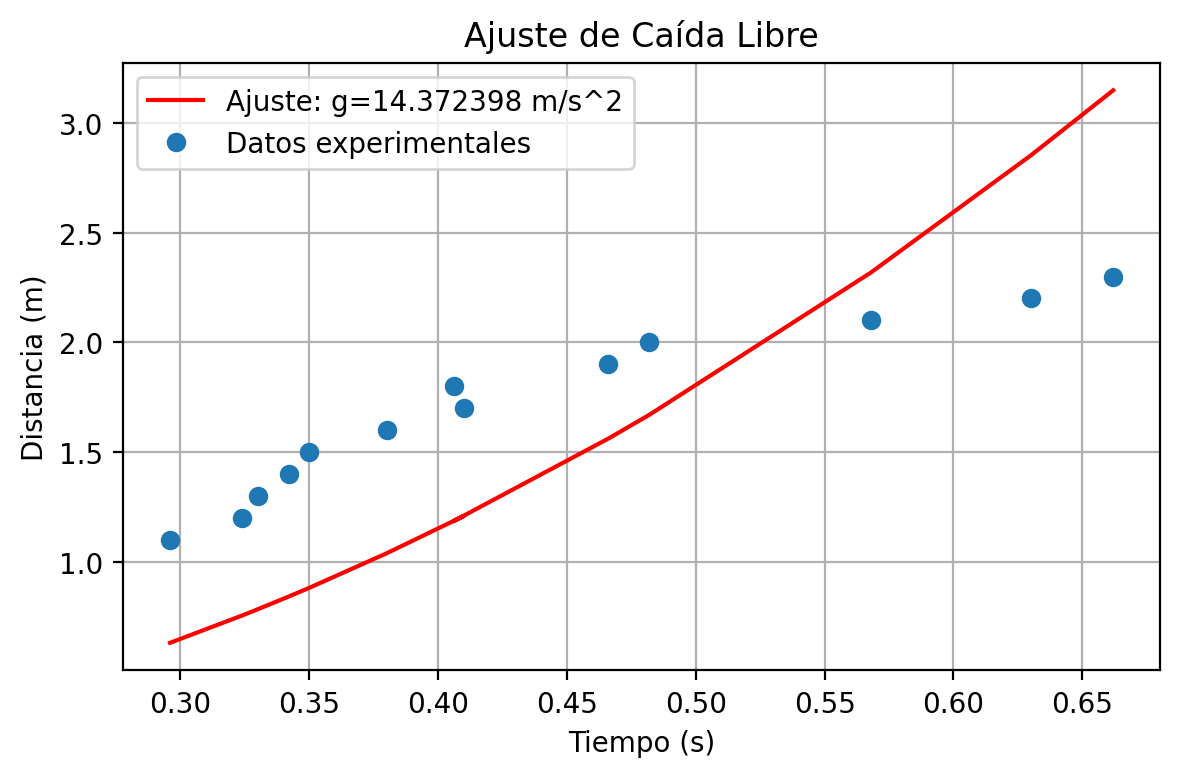
\includegraphics[width=0.6\linewidth]{imgs/ajuste_caida.png}
    \caption{Curva de ajuste superpuesta a los datos experimentales.}
    \label{fig:ajuste}
\end{figure}

Al observar la gráfica de ajuste (Figura \ref{fig:ajuste}), es claro que la dispersión de los datos no fluye de manera natural desde el origen $(0,0)$. Aunque la pelota efectivamente se soltó desde el reposo en el tiempo exacto $t=0$, el uso de cronómetros manuales introdujo demoras de activación o detención en la lectura del tiempo (es decir, el tiempo de reacción en el usuario al activar o pausar el reloj). 

Dado que el modelo programado asume que el objeto empieza a caer y registrar el tiempo instantáneamente forzando la curva desde el origen numéricamente, y que además los tiempos manuales están alterados, el algoritmo de mínimos cuadrados se ve obligado a aumentar drásticamente la concavidad de la parábola para tratar de ``atrapar'' los puntos experimentales. Esto se traduce directamente en un parámetro $g$ totalmente sobreestimado.

Para cuantificar esta desviación, se calcularon los residuos de las mediciones, que corresponden a la diferencia entre los valores de $y$ experimentales y las distancias predecidas por el modelo ($y_{\text{model}}$).

\begin{table}[H]
\centering
\caption{Residuos obtenidos en el experimento de caída libre}
\label{tab:residuos_caida}
\begin{tabular}{rrrr}
\toprule
$t$ (s) & $y$ (m) & $y_{\text{model}}$ (m) & Residuo (m) \\
\midrule
0.662000 & 2.300000 & 3.149300 & -0.849300 \\
0.630000 & 2.200000 & 2.852200 & -0.652200 \\
0.568000 & 2.100000 & 2.318400 & -0.218400 \\
0.482000 & 2.000000 & 1.669500 & 0.330500 \\
0.466000 & 1.900000 & 1.560500 & 0.339500 \\
0.406000 & 1.800000 & 1.184500 & 0.615500 \\
0.410000 & 1.700000 & 1.208000 & 0.492000 \\
0.380000 & 1.600000 & 1.037700 & 0.562300 \\
0.350000 & 1.500000 & 0.880300 & 0.619700 \\
0.342000 & 1.400000 & 0.840500 & 0.559500 \\
0.330000 & 1.300000 & 0.782600 & 0.517400 \\
0.324000 & 1.200000 & 0.754400 & 0.445600 \\
0.296000 & 1.100000 & 0.629600 & 0.470400 \\
\bottomrule
\end{tabular}
\end{table}

Los residuos presentados en la Tabla \ref{tab:residuos_caida} no se distribuyen alrededor de cero de manera aleatoria (hacia arriba o hacia debajo de la curva). En su lugar, muestran un llamativo patrón de sesgo sistemático: los errores cambian consecutivamente de positivos a negativos en función del tiempo. 

Esto es una prueba indudable de los efectos de la reacción manual humana: el retraso cronométrico incrusta un desplazamiento sistemático en la variable independiente que el modelo teórico rígido de $y=\frac{g}{2}t^2$ es incapaz de asimilar. Es decir, aunque las fórmulas reflejan la física teórica correcta desde el origen, no pueden compensar este sesgo instrumental/humano si no se les programa un término adicional que permita absorber ese offset de reacción que contamina los datos.

Como consecuencia directa de este corte cronométrico intencionalmente corto por la manipulación, si analizamos la física implicada detrás de estas franjas de tiempo, encontraríamos resultados sumamente defectuosos. Por ejemplo, al validar que el objeto descendió hasta $1.6\text{ m}$ en apenas $0.380\text{ s}$ o hasta $2.3\text{ m}$ en $0.662\text{ s}$, el modelo sugiere implícitamente picos de velocidad irracionales e ``hipersónicas'' para un objeto simple en caída libre soltado a esas alturas. Dicha incoherencia subraya matemáticamente que el cuerpo físico jamás pudo haber recorrido esas distancias en esos intervalos de tiempo sin una fuerte propulsión adicional, confirmando contundentemente que la medición del reloj carece de fidelidad temporal real.

\vspace{1cm}
\section{Conclusiones}
El análisis demuestra de primera mano cómo una fuente de error experimental no mitigada durante la toma de datos puede desviar completamente una correlación numérica en la programación, sin importar cuán exacto resulte el modelo físico de sus leyes en el código. El planteamiento de estudiar un objeto en descenso desde el reposo está correctamente soportado por la cinemática de $y=\frac{g}{2}t^2$; sin embargo, es la fuerte manipulación manual con cronómetros la protagonista. 

La latencia humana intrínseca al presionar o detener el cronómetro incorporó un \textit{offset} sistemático en cada par ordenado del set de prueba. Aunque las herramientas y algoritmos numéricos como los de \texttt{scipy.optimize} minimizan funciones de error de manera robusta, matemáticamente se limitan a seguir un modelo específico hasta las últimas consecuencias. 

A falta de un factor corrector de tiempo introducido en el modelo, la parábola programada debió deformarse para encajar un juego de datos sesgado junto a una base obligada a salir del origen absoluto; sobrepasando enormemente el valor natural esperado de la aceleración a unos inviables $\approx14.37\ \mathrm{m/s^2}$. 

\end{document}
